\documentclass[tikz,border=2pt]{standalone}
\usepackage{amsmath,amssymb}
\usepackage{tikz}
\usetikzlibrary{arrows.meta}

\begin{document}
% The Euclidean norm is the length of the arrow: Pythagoras on the coordinates.
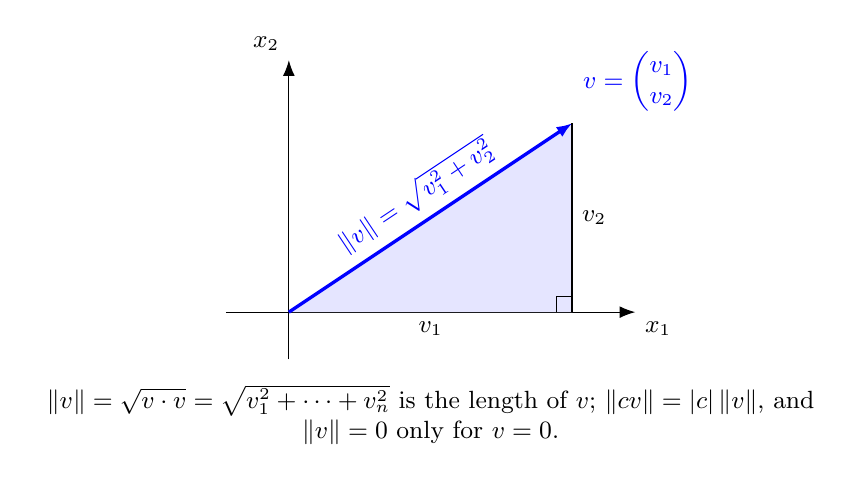
\begin{tikzpicture}[every node/.style={font=\small}, >={Latex[length=2mm]}]
	\draw[->] (-0.8,0) -- (4.4,0) node[below right] {$x_1$};
	\draw[->] (0,-0.6) -- (0,3.2) node[above left] {$x_2$};
	\fill[blue!10] (0,0) -- (3.6,0) -- (3.6,2.4) -- cycle;
	\draw[->, blue, very thick] (0,0) -- (3.6,2.4) node[midway, above, sloped] {$\|v\|=\sqrt{v_1^2+v_2^2}$} node[above right] {$v=\begin{pmatrix}v_1\\v_2\end{pmatrix}$};
	\draw[thick] (3.6,0) -- (3.6,2.4);
	\draw (3.4,0) -- (3.4,0.2) -- (3.6,0.2);
	\node[below] at (1.8,0) {$v_1$};
	\node[right] at (3.6,1.2) {$v_2$};
	\node[anchor=north, align=flush center, text width=10cm] at (1.8,-0.8) {$\|v\|=\sqrt{v\cdot v}=\sqrt{v_1^2+\cdots+v_n^2}$ is the length of $v$; $\|cv\|=|c|\,\|v\|$, and $\|v\|=0$ only for $v=0$.};
\end{tikzpicture}
\end{document}
